%=======================================================================
%  CHAPTER 6 — MACHINE LEARNING : SOLVED PROBLEMS
%=======================================================================
\section{Machine Learning \textcolor{sub}{\large -- Solved Problems}}

{\color{sub}\footnotesize Every problem opens with the question
\mk{exactly as the paper prints it}, data table and all, so it can be
attempted from this document alone. \gap$\cdot$\gap \textbf{Three ID3 data tables over
six papers}, \textbf{three genetic-algorithm runs}, and the \textbf{fuzzy arithmetic}.
\gap$\cdot$\gap Every entropy, gain, fitness value and membership number printed here is
recomputed independently by \code{verify.py}; 242 checks pass across the subject.}

\lead{\mk{Two things to know before you start.}}
\begin{itemize}
  \item \mk{The two ``play'' tables have different answers.} They look
        the same $-$ fourteen rows, same four attributes, nine Yes and five No. But
        \yr{79 Jth} changes four rows, and that moves the root attribute from
        \textbf{Outlook} to \textbf{Windy}. Copying the golf answer into the cricket
        question loses the whole 7 marks. Problems 1.1 and 1.2 are printed side by side
        for exactly this reason.
  \item \mk{\yr{\textbf{75 Bh}} prints no chromosomes.} The question
        sets up the fitness function, says \emph{``the initial population consist of four
        individuals with the following chromosomes''} $-$ and then the page runs on to
        Q7. Problem 2.2 reproduces the defect as printed and works the standard four
        chromosomes that the textbook version of this question carries.
\end{itemize}

\hr

%=======================================================================
\T{6.N.1 Decision trees: the method, used identically in all four problems}

\lead{The recipe}
\begin{itemize}
  \item \textbf{Step 1.} Count the classes in the whole set $S$. Write $P$ (positives)
        and $N$ (negatives), then
        $H(S) = -\frac{P}{P+N}\log_2\frac{P}{P+N} - \frac{N}{P+N}\log_2\frac{N}{P+N}$.
  \item \textbf{Step 2.} For each attribute, split $S$ by its values and fill \emph{one
        row per value} of the table below: the counts, that branch's entropy, and the
        branch weighted by its share of $S$.
  \item \textbf{Step 3.} Sum the weighted column. That is the \textbf{residual entropy}
        after splitting on that attribute.
  \item \textbf{Step 4.} $Gain = H(S) - $ residual. Compare the gains; the largest wins.
  \item \textbf{Step 5.} Recurse on each branch that is not already pure.
\end{itemize}

\lead{The table idiom, used unchanged in every problem below}
\begin{tabularx}{\textwidth}{@{}L{2.1cm}L{1.9cm}ccccX@{}}
\hrow \thead{Attribute} & \thead{Value} & \thead{$P$} & \thead{$N$} &
  \thead{$|S_v|$} & \thead{$H(S_v)$} & \thead{$\frac{|S_v|}{|S|}H(S_v)$} \\
\end{tabularx}

\lead{Two logarithms are all you ever need}
{\color{sub}\footnotesize $\log_2 x = \frac{\ln x}{\ln 2}$, and these five cover every
split in this chapter.}
\begin{tabularx}{\textwidth}{@{}L{4.2cm}XXXXX@{}}
\hrow \thead{Split $P$:$N$} & \thead{1:1} & \thead{1:2 or 2:1} & \thead{1:3 or 3:1} &
  \thead{2:3 or 3:2} & \thead{3:4 or 4:3} \\
$H$ & 1.0000 & 0.9183 & 0.8113 & 0.9710 & 0.9852 \\
\end{tabularx}
{\color{sub}\footnotesize Also $H(1{:}6)=0.5917$, $H(2{:}5)=0.8631$, $H(5{:}9)=0.9403$,
$H(3{:}5)=0.9544$, and $H=0$ whenever one side is empty.}

%=======================================================================
\T{6.N.2 Problem 1.1 --- the ``play golf'' table (3 papers)}

\creamq{Select the root attribute of the decision tree from the given sample data}{\m{8}\m{2+7}}
{\color{sub}\footnotesize \tP{3} \yr{\textbf{\textit{74 Bh}} \m{2+7},
\textit{74 Ma} \m{8}, \textbf{\textit{72 Ash}} \m{8}} \gap$\cdot$\gap all three print the
\emph{same} fourteen rows \gap$\cdot$\gap \yr{\textbf{\textit{74 Bh}}} asks for the ID3
approach first, which is \S6.5}

\begin{asked}{\textbf{\textit{74 Bh}} \textperiodcentered{} Q4 \textperiodcentered{} \m{2+7}}
State the approach for learning using ID3 and Select the root attribute of the
decision-tree from given sample data.
\par\penalty0\vspace{2pt}
\begin{tabularx}{0.86\linewidth}{@{}XXXXX@{}}
\hrow \thead{Outlook} & \thead{Temperature} & \thead{Humidity} & \thead{Windy} &
  \thead{Play golf} \\
Rainy & Hot & High & False & No \\
Rainy & Hot & High & True & No \\
Overcast & Hot & High & False & Yes \\
Sunny & Mild & High & False & Yes \\
Sunny & Cool & Normal & False & Yes \\
Sunny & Cool & Normal & True & No \\
Overcast & Cool & Normal & True & Yes \\
Rainy & Mild & High & False & No \\
Rainy & Cool & Normal & False & Yes \\
Sunny & Mild & Normal & False & Yes \\
Rainy & Mild & Normal & True & Yes \\
Overcast & Mild & High & True & Yes \\
Overcast & Hot & Normal & False & Yes \\
Sunny & Mild & High & True & No \\
\end{tabularx}
\end{asked}

\lead{Step 1 \gap Entropy of the whole set}
{\color{sub}\footnotesize 14 rows: \textbf{9 Yes}, \textbf{5 No}.}
\[ H(S) = -\frac{9}{14}\log_2\frac{9}{14} - \frac{5}{14}\log_2\frac{5}{14}
        = 0.4098 + 0.5305 = \mathbf{0.9403} \]

\lead{Steps 2 and 3 \gap Split on each attribute in turn}
\begin{tabularx}{\textwidth}{@{}L{2.1cm}L{1.9cm}ccccX@{}}
\hrow \thead{Attribute} & \thead{Value} & \thead{$P$} & \thead{$N$} &
  \thead{$|S_v|$} & \thead{$H(S_v)$} & \thead{$\frac{|S_v|}{14}H(S_v)$} \\
\textbf{Outlook} & Rainy    & 2 & 3 & 5 & 0.9710 & $\frac{5}{14}(0.9710)=0.3468$ \\
                 & Overcast & 4 & 0 & 4 & \mk{0} & 0 \\
                 & Sunny    & 3 & 2 & 5 & 0.9710 & $\frac{5}{14}(0.9710)=0.3468$ \\
\hrow \multicolumn{6}{@{}l}{residual $=0.6935$} & \mk{Gain $=0.9403-0.6935=0.2467$} \\
Temperature & Hot  & 2 & 2 & 4 & 1.0000 & 0.2857 \\
            & Mild & 4 & 2 & 6 & 0.9183 & 0.3936 \\
            & Cool & 3 & 1 & 4 & 0.8113 & 0.2318 \\
\hrow \multicolumn{6}{@{}l}{residual $=0.9111$} & Gain $=0.0292$ \\
Humidity & High   & 3 & 4 & 7 & 0.9852 & 0.4926 \\
         & Normal & 6 & 1 & 7 & 0.5917 & 0.2958 \\
\hrow \multicolumn{6}{@{}l}{residual $=0.7885$} & Gain $=0.1518$ \\
Windy & False & 6 & 2 & 8 & 0.8113 & 0.4636 \\
      & True  & 3 & 3 & 6 & 1.0000 & 0.4286 \\
\hrow \multicolumn{6}{@{}l}{residual $=0.8922$} & Gain $=0.0481$ \\
\end{tabularx}

\sbsr{0.48}{%
\lead{Step 4 \gap Compare}
\begin{tabularx}{\linewidth}{@{}L{3.0cm}X@{}}
\hrow \thead{Attribute} & \thead{Gain} \\
\mk{Outlook} & \mk{0.2467} \\
Humidity & 0.1518 \\
Windy & 0.0481 \\
Temperature & 0.0292 \\
\end{tabularx}
\par\penalty0\vspace{3pt}
\noindent\colorbox{gdL}{\parbox{\dimexpr\linewidth-2\fboxsep}{\textbf{Answer.} The root
attribute is \textbf{Outlook}, with the highest information gain, \textbf{0.2467}.}}}{%
\lead{Why Outlook wins}
\begin{itemize}
  \item Outlook is the only attribute with a \mk{pure branch} $-$ all four
        \emph{Overcast} days are Yes $-$ so it removes more uncertainty than any other.
  \item Temperature removes almost none: its three branches are as mixed as the parent.
  \item \textbf{Overcast} (rows 3, 7, 12, 13) is all Yes, so it becomes a
        \mk{leaf} at once. \textbf{Rainy} (2:3) and \textbf{Sunny} (3:2) both still
        have $H=0.9710$, so each needs its own split: Step 5.
\end{itemize}}

\lead{Step 5 \gap Recurse: Steps 1 to 4 again, inside each impure branch \gap{\color{sub}\footnotesize(not asked, but it proves the root was right)}}
{\color{sub}\footnotesize Rows numbered 1 to 14 top to bottom. Each branch uses only
\emph{its own} five rows and only the three attributes Outlook has not used. Both
branches start from $H=0.9710$, so the residual is the whole story.}
\sbs{%
\textbf{Outlook $=$ Rainy} {\color{sub}\footnotesize rows 1, 2, 8, 9, 11 \gap 2 Yes, 3 No}
\par\vspace{2pt}
\begin{tabularx}{\linewidth}{@{}l@{\hspace{5pt}}lcccX@{}}
\hrow \thead{Attribute} & \thead{Value (rows)} & \thead{$P$} & \thead{$N$} &
  \thead{$H$} & \thead{Gain} \\
\textbf{Humidity} & High (1,2,8) & 0 & 3 & \mk{0} & \\
                  & Normal (9,11) & 2 & 0 & \mk{0} & \mk{0.9710} \\
\hrow Temperature & Hot (1,2)  & 0 & 2 & 0 & \\
                  & Mild (8,11) & 1 & 1 & 1.0000 & \\
                  & Cool (9)   & 1 & 0 & 0 & 0.5710 \\
\hrow Windy & False (1,8,9) & 1 & 2 & 0.9183 & \\
            & True (2,11)   & 1 & 1 & 1.0000 & 0.0200 \\
\end{tabularx}
\par\vspace{2pt}
{\footnotesize Humidity: residual $0$, gain $=0.9710-0=0.9710$. Temperature: residual
$\frac{2}{5}(1)=0.4000$, gain $0.5710$. Windy: residual
$\frac{3}{5}(0.9183)+\frac{2}{5}(1)=0.9510$, gain $0.0200$. \mk{Split on Humidity.}}}{%
\textbf{Outlook $=$ Sunny} {\color{sub}\footnotesize rows 4, 5, 6, 10, 14 \gap 3 Yes, 2 No}
\par\vspace{2pt}
\begin{tabularx}{\linewidth}{@{}l@{\hspace{5pt}}lcccX@{}}
\hrow \thead{Attribute} & \thead{Value (rows)} & \thead{$P$} & \thead{$N$} &
  \thead{$H$} & \thead{Gain} \\
\textbf{Windy} & False (4,5,10) & 3 & 0 & \mk{0} & \\
               & True (6,14)    & 0 & 2 & \mk{0} & \mk{0.9710} \\
\hrow Temperature & Mild (4,10,14) & 2 & 1 & 0.9183 & \\
                  & Cool (5,6)     & 1 & 1 & 1.0000 & 0.0200 \\
\hrow Humidity & High (4,14)    & 1 & 1 & 1.0000 & \\
               & Normal (5,6,10) & 2 & 1 & 0.9183 & 0.0200 \\
\end{tabularx}
\par\vspace{2pt}
{\footnotesize Windy: residual $0$, gain $0.9710$. Temperature and Humidity each leave
one 1:1 pair and one 2:1 triple: residual $\frac{2}{5}(1)+\frac{3}{5}(0.9183)=0.9510$,
gain $0.0200$. \mk{Split on Windy.}}}

\par\vspace{2pt}
\noindent\textbf{The tree}, three levels and five leaves, one rule per leaf:
\code{Outlook = Overcast -> Yes}; \code{Outlook = Rainy, Humidity = High -> No};
\code{Outlook = Rainy, Humidity = Normal -> Yes}; \code{Outlook = Sunny, Windy = False -> Yes};
\code{Outlook = Sunny, Windy = True -> No}. Temperature never appears:
\mk{ID3 has decided it is irrelevant}, which is the feature-selection side of the algorithm.
% ch6fig:slot c6_tree_golf
% ch6fig:c6_tree_golf (generated by ch6fig.py; do not edit)
\penalty0\vspace{3pt}
\Needspace{235pt}
\lead{The finished tree: play golf (rows numbered 1 to 14 top to bottom)}
\begin{center}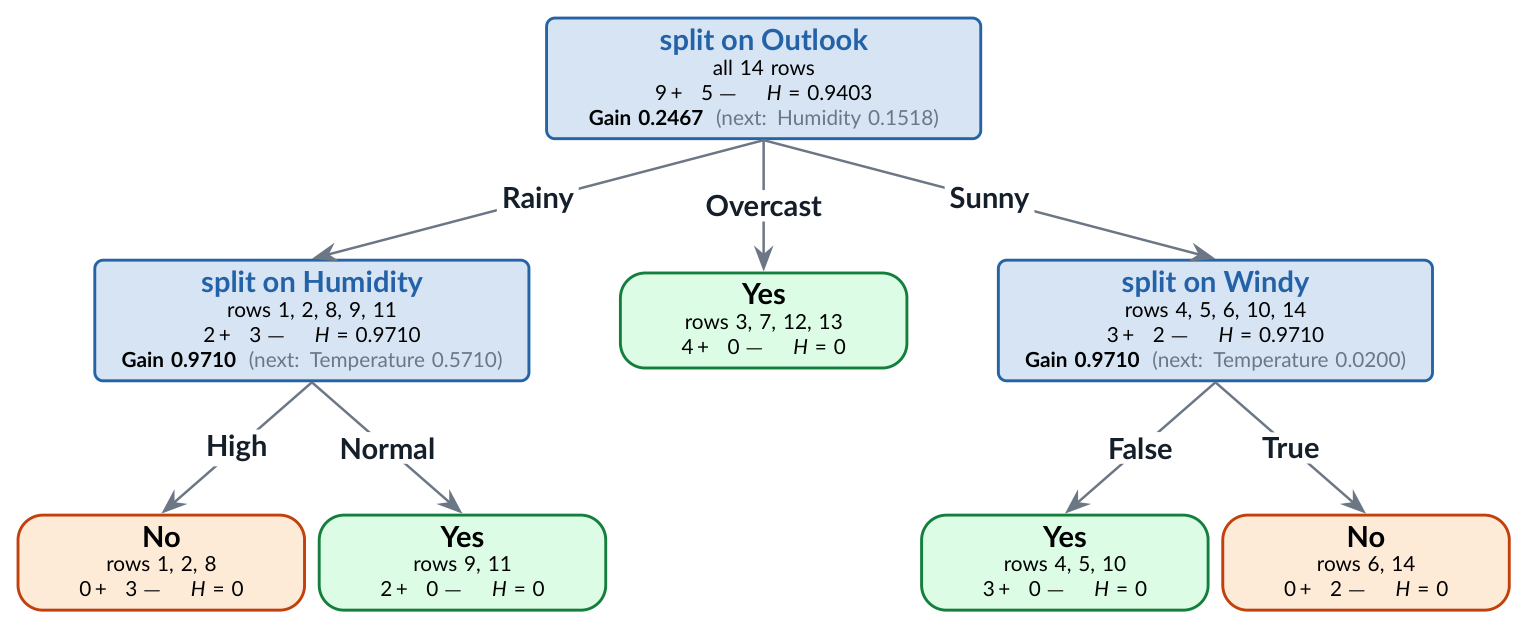
\includegraphics[width=513.2pt]{figs/c6_tree_golf.png}\end{center}
\par\Needspace{16\baselineskip}
% ch6fig:end
%=======================================================================
\T{6.N.3 Problem 1.2 --- the ``play cricket'' table, whose answer is different}

\creamq{How is the best attribute selected in a decision tree? Select the root attribute from the given sample data}{\m{1+7}}
{\color{sub}\footnotesize \yr{79 Jth} \m{1+7} \gap$\cdot$\gap
\mk{four rows differ from Problem 1.1 and the answer changes}
\gap$\cdot$\gap rows 1 and 11 carry a different label, row 8 a different \emph{Windy}
value, and the target is renamed \emph{Play cricket}}

\begin{asked}{79 Jth \textperiodcentered{} Q8b \textperiodcentered{} \m{1+7}}
How best attribute is selected in a decision-tree? Select the root attribute of the
decision-tree from given sample data.
\par\penalty0\vspace{2pt}
\begin{tabularx}{0.86\linewidth}{@{}XXXXX@{}}
\hrow \thead{Outlook} & \thead{Temperature} & \thead{Humidity} & \thead{Windy} &
  \thead{Play cricket} \\
Rainy & Hot & High & False & \mk{Yes} \\
Rainy & Hot & High & True & No \\
Overcast & Hot & High & False & Yes \\
Sunny & Mild & High & False & Yes \\
Sunny & Cool & Normal & False & Yes \\
Sunny & Cool & Normal & True & No \\
Overcast & Cool & Normal & True & Yes \\
Rainy & Mild & High & \mk{True} & No \\
Rainy & Cool & Normal & False & Yes \\
Sunny & Mild & Normal & False & Yes \\
Rainy & Mild & Normal & True & \mk{No} \\
Overcast & Mild & High & True & Yes \\
Overcast & Hot & Normal & False & Yes \\
Sunny & Mild & High & True & No \\
\end{tabularx}
\end{asked}

\lead{Step 1 \gap Entropy of the whole set}
{\color{sub}\footnotesize Still \textbf{9 Yes} and \textbf{5 No} out of 14, so
$H(S)=\mathbf{0.9403}$ again $-$ which is exactly why the table looks identical.}

\lead{Steps 2 and 3}
\begin{tabularx}{\textwidth}{@{}L{2.1cm}L{1.9cm}ccccX@{}}
\hrow \thead{Attribute} & \thead{Value} & \thead{$P$} & \thead{$N$} &
  \thead{$|S_v|$} & \thead{$H(S_v)$} & \thead{$\frac{|S_v|}{14}H(S_v)$} \\
\textbf{Windy} & False & 7 & 0 & 7 & \mk{0} & 0 \\
               & True  & 2 & 5 & 7 & 0.8631 & $\frac{7}{14}(0.8631)=0.4316$ \\
\hrow \multicolumn{6}{@{}l}{residual $=0.4316$} & \mk{Gain $=0.9403-0.4316=0.5087$} \\
Outlook & Rainy    & 2 & 3 & 5 & 0.9710 & 0.3468 \\
        & Overcast & 4 & 0 & 4 & 0      & 0 \\
        & Sunny    & 3 & 2 & 5 & 0.9710 & 0.3468 \\
\hrow \multicolumn{6}{@{}l}{residual $=0.6935$} & Gain $=0.2467$ \\
Temperature & Hot  & 3 & 1 & 4 & 0.8113 & 0.2318 \\
            & Mild & 3 & 3 & 6 & 1.0000 & 0.4286 \\
            & Cool & 3 & 1 & 4 & 0.8113 & 0.2318 \\
\hrow \multicolumn{6}{@{}l}{residual $=0.8922$} & Gain $=0.0481$ \\
Humidity & High   & 4 & 3 & 7 & 0.9852 & 0.4926 \\
         & Normal & 5 & 2 & 7 & 0.8631 & 0.4316 \\
\hrow \multicolumn{6}{@{}l}{residual $=0.9242$} & Gain $=0.0161$ \\
\end{tabularx}

\sbsr{0.46}{%
\par\penalty0\vspace{2pt}
\noindent\colorbox{gdL}{\parbox{\dimexpr\linewidth-2\fboxsep}{\textbf{Answer.} The root
attribute is \textbf{Windy}, gain \textbf{0.5087} $-$ more than twice Outlook's 0.2467.}}
\begin{itemize}
  \item \mk{Compare with Problem 1.1, where Windy was the second
        \emph{worst} attribute at 0.0481.} Three changed labels turned it into the
        best one.
  \item \textbf{Why}: in this table \mk{every one of the seven
        non-windy days is a Yes}. One branch of Windy is completely pure and holds
        half the data, which is the largest single reduction in uncertainty available.
  \item \mk{The lesson worth writing in the answer}: never carry a
        remembered root across from a similar-looking table. Recompute.
\end{itemize}}{%
\lead{Finishing the tree \gap{\color{sub}\footnotesize(it is only two levels deep)}}
\begin{itemize}
  \item \textbf{Windy $=$ False} $-$ rows 1, 3, 4, 5, 9, 10, 13, all Yes. \mk{Leaf: Yes.}
  \item \textbf{Windy $=$ True} $-$ rows 2, 6, 7, 8, 11, 12, 14: 2 Yes 5 No, $H=0.8631$.
        Steps 1 to 4 again on those seven rows, with the three attributes left:
\end{itemize}
\begin{tabularx}{\linewidth}{@{}l@{\hspace{5pt}}lcccX@{}}
\hrow \thead{Attribute} & \thead{Value (rows)} & \thead{$P$} & \thead{$N$} &
  \thead{$H$} & \thead{Gain} \\
\textbf{Outlook} & Rainy (2,8,11)  & 0 & 3 & \mk{0} & \\
                 & Sunny (6,14)    & 0 & 2 & \mk{0} & \\
                 & Overcast (7,12) & 2 & 0 & \mk{0} & \mk{0.8631} \\
\hrow Temperature & Hot (2)            & 0 & 1 & 0 & \\
                  & Cool (6,7)         & 1 & 1 & 1.0000 & \\
                  & Mild (8,11,12,14)  & 1 & 3 & 0.8113 & 0.1138 \\
\hrow Humidity & High (2,8,12,14) & 1 & 3 & 0.8113 & \\
               & Normal (6,7,11)  & 1 & 2 & 0.9183 & 0.0060 \\
\end{tabularx}
\par\vspace{2pt}
{\footnotesize Outlook: every branch pure, residual $0$, gain $=0.8631$. Temperature:
residual $\frac{2}{7}(1)+\frac{4}{7}(0.8113)=0.7493$, gain $0.1138$. Humidity: residual
$\frac{4}{7}(0.8113)+\frac{3}{7}(0.9183)=0.8571$, gain $0.0060$. \mk{Split on Outlook.}}}

\par\vspace{2pt}
\begin{itemize}
  \item \textbf{The tree}, four leaves and only two tests:
        \code{Windy = False -> Yes}; \code{Windy = True, Outlook = Rainy -> No};
        \code{Windy = True, Outlook = Sunny -> No};
        \code{Windy = True, Outlook = Overcast -> Yes}.
  \item Neither Temperature nor Humidity is ever tested. The cricket tree is
        \mk{smaller than the golf tree} $-$ two tests against three $-$
        which is what a higher root gain buys you.
\end{itemize}
% ch6fig:slot c6_tree_cricket
% ch6fig:c6_tree_cricket (generated by ch6fig.py; do not edit)
\penalty0\vspace{3pt}
\Needspace{235pt}
\lead{The finished tree: play cricket, two tests instead of three}
\begin{center}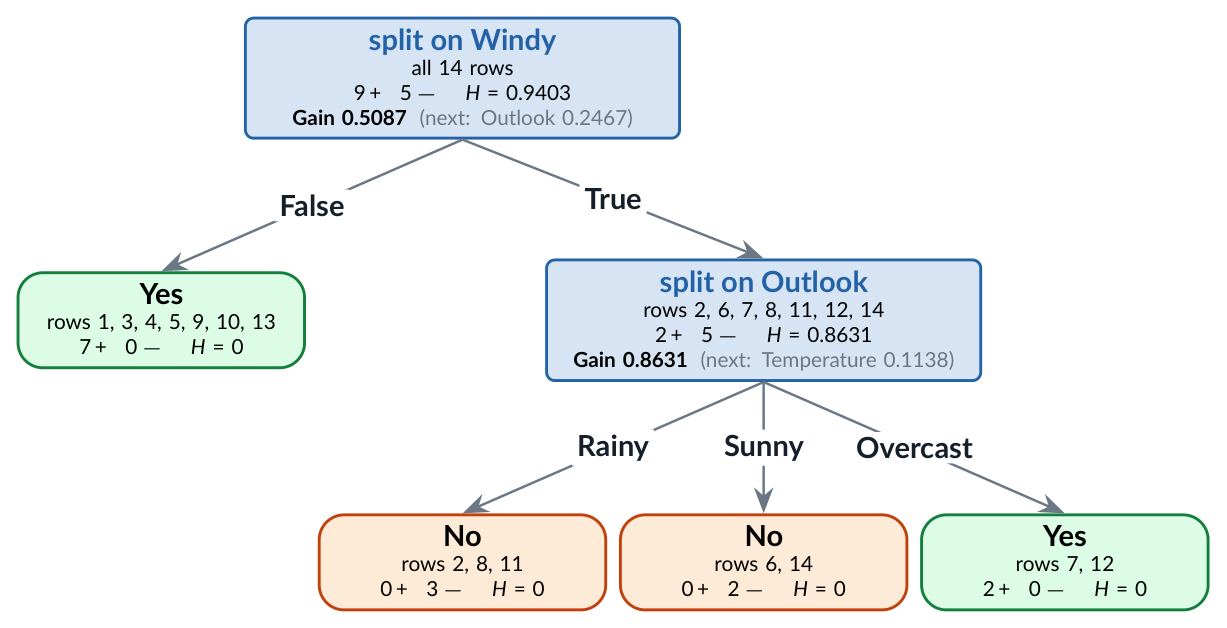
\includegraphics[width=412.0pt]{figs/c6_tree_cricket.png}\end{center}
\par\Needspace{16\baselineskip}
% ch6fig:end
%=======================================================================
\T{6.N.4 Problem 1.3 --- the mushroom island}

\creamq{Which attribute should you choose as the root of a decision tree? Give reason}{\m{8}}
{\color{sub}\footnotesize \yr{\textbf{\textit{77 Ch}}} \m{8} \gap$\cdot$\gap
the attributes are already 0/1, so no entropy is wasted on multi-way splits
\gap$\cdot$\gap \mk{only A to H are training data}; U, V and W carry
\emph{?} in the Edible column and are the cases to be classified afterwards}

\begin{asked}{\textbf{\textit{77 Ch}} \textperiodcentered{} Q7 \textperiodcentered{} \m{8}}
You are locked on a deserted island. Mushrooms of various types grow widely all over the
island but no other food is anywhere to be found. Some of the mushrooms have been
determined as poisonous and others as not (Determined by your former companions' trial
and error). You are the only on reaming on the island. You have the following data to
consider;
\par\penalty0\vspace{2pt}
\begin{tabularx}{0.80\linewidth}{@{}XXXXXX@{}}
\hrow \thead{Example} & \thead{NotHeavy} & \thead{Smelly} & \thead{Spotted} &
  \thead{Smooth} & \thead{Edible} \\
A & 1 & 0 & 0 & 0 & 1 \\
B & 1 & 0 & 1 & 0 & 1 \\
C & 0 & 1 & 0 & 1 & 1 \\
D & 0 & 0 & 0 & 1 & 0 \\
E & 1 & 1 & 1 & 0 & 0 \\
F & 1 & 0 & 1 & 1 & 0 \\
G & 1 & 0 & 0 & 1 & 0 \\
H & 0 & 1 & 0 & 0 & 0 \\
U & 0 & 1 & 1 & 1 & ? \\
V & 1 & 1 & 0 & 1 & ? \\
W & 1 & 1 & 0 & 0 & ? \\
\end{tabularx}
\par\penalty0\vspace{2pt}
You know whether or not mushroom A through H are poisonous, but you do not know about U
through W. Which attributes should you choose as the root of a decision tree? Give
reason.
\par\penalty0\vspace{1pt}
{\color{sub}\footnotesize The paper's own wording, slips included:
``the only on reaming'' for \emph{the only one remaining}.}
\end{asked}

\lead{Step 1 \gap Entropy of the training set}
{\color{sub}\footnotesize Rows A--H only. Edible $=1$ for \textbf{A, B, C}
$\rightarrow P=3$; Edible $=0$ for \textbf{D, E, F, G, H} $\rightarrow N=5$.}
\[ H(S) = -\frac{3}{8}\log_2\frac{3}{8} - \frac{5}{8}\log_2\frac{5}{8}
        = 0.5306 + 0.4238 = \mathbf{0.9544} \]

\lead{Steps 2 and 3 \gap All four attributes}
\begin{tabularx}{\textwidth}{@{}L{2.1cm}L{2.6cm}ccccX@{}}
\hrow \thead{Attribute} & \thead{Value (rows)} & \thead{$P$} & \thead{$N$} &
  \thead{$|S_v|$} & \thead{$H(S_v)$} & \thead{$\frac{|S_v|}{8}H(S_v)$} \\
\textbf{Smooth} & 1 (C,D,F,G) & 1 & 3 & 4 & 0.8113 & 0.4056 \\
                & 0 (A,B,E,H) & 2 & 2 & 4 & 1.0000 & 0.5000 \\
\hrow \multicolumn{6}{@{}l}{residual $=0.9056$} & \mk{Gain $=0.0488$} \\
NotHeavy & 1 (A,B,E,F,G) & 2 & 3 & 5 & 0.9710 & 0.6069 \\
         & 0 (C,D,H)     & 1 & 2 & 3 & 0.9183 & 0.3444 \\
\hrow \multicolumn{6}{@{}l}{residual $=0.9512$} & Gain $=0.0032$ \\
Smelly & 1 (C,E,H)       & 1 & 2 & 3 & 0.9183 & 0.3444 \\
       & 0 (A,B,D,F,G)   & 2 & 3 & 5 & 0.9710 & 0.6069 \\
\hrow \multicolumn{6}{@{}l}{residual $=0.9512$} & Gain $=0.0032$ \\
Spotted & 1 (B,E,F)      & 1 & 2 & 3 & 0.9183 & 0.3444 \\
        & 0 (A,C,D,G,H)  & 2 & 3 & 5 & 0.9710 & 0.6069 \\
\hrow \multicolumn{6}{@{}l}{residual $=0.9512$} & Gain $=0.0032$ \\
\end{tabularx}

\sbsr{0.50}{%
\par\penalty0\vspace{2pt}
\noindent\colorbox{gdL}{\parbox{\dimexpr\linewidth-2\fboxsep}{\textbf{Answer.} Choose
\textbf{Smooth} as the root: gain \textbf{0.0488}, fifteen times the gain of any other
attribute.}}
\lead{The reason the question asks for}
\begin{itemize}
  \item Smooth is the only attribute that produces an \textbf{uneven} class split:
        of the four smooth mushrooms only one is edible (3:1), while the four
        non-smooth ones are an even 2:2.
  \item \mk{The other three attributes split the data identically}
        $-$ each one puts 1 edible and 2 inedible on one side and 2 edible and 3
        inedible on the other, so all three have exactly the same entropy and exactly
        the same gain, 0.0032. Say this: it is the observation the examiner is looking
        for, and it means the choice between those three is arbitrary.
\end{itemize}}{%
\lead{Two things worth adding for the last marks}
\begin{itemize}
  \item \mk{No attribute here is much use at the root.} The best gain is 0.0488
        against a starting entropy of 0.9544, so the root removes only about
        \textbf{5\,\%} of the uncertainty.
  \item \mk{But the second level is perfect.} Under either value of Smooth,
        \textbf{Smelly} separates the mushrooms completely (tables below). The tree
        is therefore only two tests deep, and it classifies U, V and W: the story
        implies that even though the question stops at the root.
  \item Beware the root-only shortcut: reading U and V off the 3:1 Smooth branch
        says \emph{not edible}, and the full tree says the opposite.
\end{itemize}}

\lead{Finishing the tree \gap{\color{sub}\footnotesize(not asked; it is how U, V and W get classified)}}
{\color{sub}\footnotesize Each branch uses only its own four mushrooms and only the three
attributes Smooth has not used.}
\sbs{%
\textbf{Smooth $=$ 0} {\color{sub}\footnotesize A, B, E, H \gap 2 edible, 2 not, $H=1$}
\par\vspace{2pt}
\begin{tabularx}{\linewidth}{@{}l@{\hspace{5pt}}lcccX@{}}
\hrow \thead{Attribute} & \thead{Value (rows)} & \thead{$P$} & \thead{$N$} &
  \thead{$H$} & \thead{Gain} \\
\textbf{Smelly} & 0 (A,B) & 2 & 0 & \mk{0} & \\
                & 1 (E,H) & 0 & 2 & \mk{0} & \mk{1.0000} \\
\hrow NotHeavy & 1 (A,B,E) & 2 & 1 & 0.9183 & \\
               & 0 (H)     & 0 & 1 & 0 & 0.3113 \\
\hrow Spotted & 1 (B,E) & 1 & 1 & 1.0000 & \\
              & 0 (A,H) & 1 & 1 & 1.0000 & 0 \\
\end{tabularx}
\par\vspace{2pt}
{\footnotesize NotHeavy: residual $\frac{3}{4}(0.9183)=0.6887$, gain $0.3113$. Spotted
leaves both halves 1:1, gain 0. \mk{Split on Smelly.}}}{%
\textbf{Smooth $=$ 1} {\color{sub}\footnotesize C, D, F, G \gap 1 edible, 3 not, $H=0.8113$}
\par\vspace{2pt}
\begin{tabularx}{\linewidth}{@{}l@{\hspace{5pt}}lcccX@{}}
\hrow \thead{Attribute} & \thead{Value (rows)} & \thead{$P$} & \thead{$N$} &
  \thead{$H$} & \thead{Gain} \\
\textbf{Smelly} & 1 (C)     & 1 & 0 & \mk{0} & \\
                & 0 (D,F,G) & 0 & 3 & \mk{0} & \mk{0.8113} \\
\hrow NotHeavy & 0 (C,D) & 1 & 1 & 1.0000 & \\
               & 1 (F,G) & 0 & 2 & 0 & 0.3113 \\
\hrow Spotted & 0 (C,D,G) & 1 & 2 & 0.9183 & \\
              & 1 (F)     & 0 & 1 & 0 & 0.1226 \\
\end{tabularx}
\par\vspace{2pt}
{\footnotesize NotHeavy: residual $\frac{2}{4}(1)=0.5000$, gain $0.3113$. Spotted: residual
$\frac{3}{4}(0.9183)=0.6887$, gain $0.1226$. \mk{Split on Smelly.}}}

\par\vspace{2pt}
\noindent\textbf{The tree}: \code{Smooth = 0, Smelly = 0 -> Edible};
\code{Smooth = 0, Smelly = 1 -> Poisonous}; \code{Smooth = 1, Smelly = 1 -> Edible};
\code{Smooth = 1, Smelly = 0 -> Poisonous}. Smelly flips meaning between the two
branches, which is why it looked useless on its own at the root.
\begin{itemize}
  \item \code{U: Smooth = 1, Smelly = 1} $\rightarrow$ predict \textbf{Edible}.
  \item \code{V: Smooth = 1, Smelly = 1} $\rightarrow$ predict \textbf{Edible}.
  \item \code{W: Smooth = 0, Smelly = 1} $\rightarrow$ predict \textbf{Poisonous}.
  \item \mk{The honest caveat}: the leaf U and V land in holds a single training
        mushroom, C. Eight examples cannot make that leaf trustworthy, so the
        answer should say the tree predicts \emph{edible} on the evidence of one
        mushroom $-$ and on an island where the cost of a wrong guess is death,
        that is a reason to abstain.
\end{itemize}
% ch6fig:slot c6_tree_mush
% ch6fig:c6_tree_mush (generated by ch6fig.py; do not edit)
\penalty0\vspace{3pt}
\Needspace{249pt}
\lead{The finished tree: the mushroom island, with U, V and W dropped through it}
\begin{center}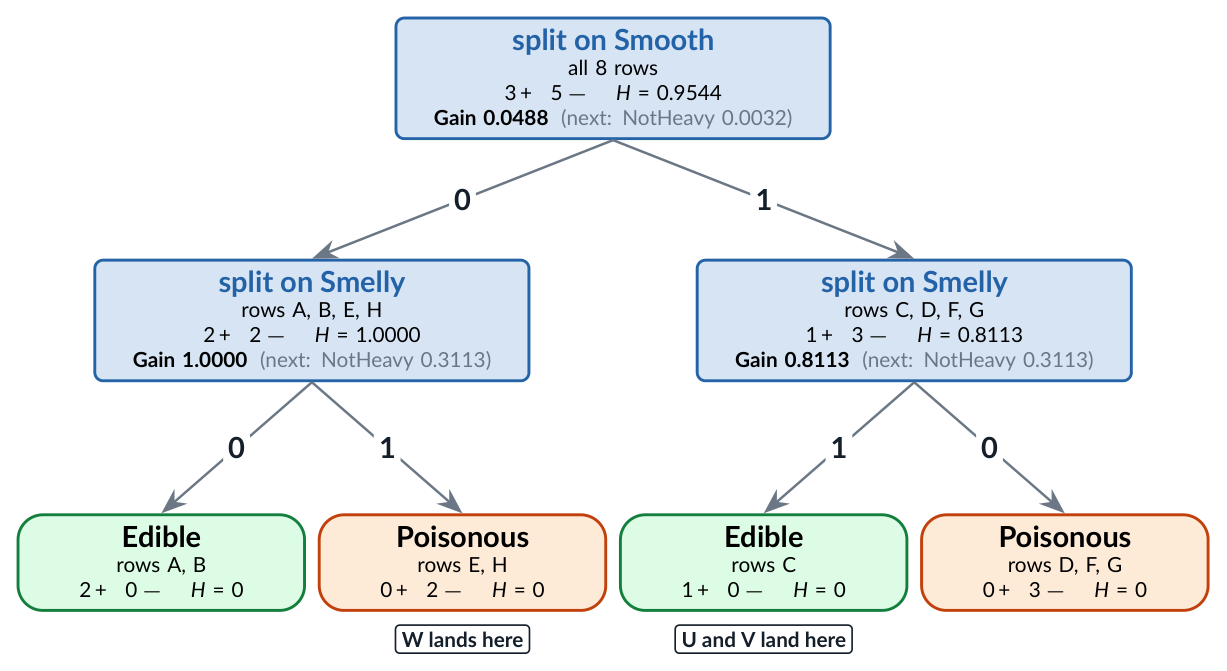
\includegraphics[width=412.0pt]{figs/c6_tree_mush.png}\end{center}
\par\Needspace{16\baselineskip}
% ch6fig:end
%=======================================================================
\T{6.N.5 Problem 1.4 --- the profit table (extra practice, not a PYQ)}

\begin{asked}[PROBLEM]{not a PYQ \textperiodcentered{} \emph{Insights} Example 6.4, the worked example the textbook uses}
Build a decision tree for the following data using ID3.
\par\penalty0\vspace{2pt}
\begin{tabularx}{0.62\linewidth}{@{}XXXX@{}}
\hrow \thead{Age} & \thead{Competition} & \thead{Type} & \thead{Profit} \\
Old & Yes & Software & Down \\
Old & No & Software & Down \\
Old & No & Hardware & Down \\
Mid & Yes & Software & Down \\
Mid & Yes & Hardware & Down \\
Mid & No & Hardware & Up \\
Mid & No & Software & Up \\
New & Yes & Software & Up \\
New & No & Hardware & Up \\
New & No & Software & Up \\
\end{tabularx}
\end{asked}

\sbsr{0.62}{%
\lead{Level 1}
{\color{sub}\footnotesize 10 rows, \textbf{5 Up} and \textbf{5 Down}, so
$H(S) = 1.0000$ exactly $-$ the easiest possible starting point.}
\begin{tabularx}{\linewidth}{@{}L{2.0cm}L{1.7cm}ccccX@{}}
\hrow \thead{Attribute} & \thead{Value} & \thead{$P$} & \thead{$N$} &
  \thead{$|S_v|$} & \thead{$H(S_v)$} & \thead{$\frac{|S_v|}{10}H$} \\
\textbf{Age} & Old & 0 & 3 & 3 & \mk{0} & 0 \\
             & Mid & 2 & 2 & 4 & 1.0000 & 0.4000 \\
             & New & 3 & 0 & 3 & \mk{0} & 0 \\
\hrow \multicolumn{6}{@{}l}{residual $=0.4000$} & \mk{Gain $=0.6000$} \\
Competition & Yes & 1 & 3 & 4 & 0.8113 & 0.3245 \\
            & No  & 4 & 2 & 6 & 0.9183 & 0.5510 \\
\hrow \multicolumn{6}{@{}l}{residual $=0.8755$} & Gain $=0.1245$ \\
Type & Software & 3 & 3 & 6 & 1.0000 & 0.6000 \\
     & Hardware & 2 & 2 & 4 & 1.0000 & 0.4000 \\
\hrow \multicolumn{6}{@{}l}{residual $=1.0000$} & Gain $=\mathbf{0}$ \\
\end{tabularx}
\begin{itemize}
  \item \mk{Type has gain exactly zero}: both its branches are split
        50/50, the same as the parent, so it tells you nothing at all. That is the
        cleanest illustration in this chapter of what a useless attribute looks like.
  \item Root $=$ \textbf{Age}. Old $\rightarrow$ Down, New $\rightarrow$ Up, both pure.
        Only \emph{Mid} needs a second level.
\end{itemize}}{%
\lead{Level 2, the Mid branch}
{\color{sub}\footnotesize 4 rows, 2 Up and 2 Down, $H=1$.}
\begin{tabularx}{\linewidth}{@{}L{2.4cm}L{1.3cm}cccX@{}}
\hrow \thead{Attribute} & \thead{Value} & \thead{$P$} & \thead{$N$} &
  \thead{$H$} & \thead{Gain} \\
\textbf{Competition} & Yes & 0 & 2 & 0 & \\
                     & No  & 2 & 0 & 0 & \mk{1.0000} \\
Type & Software & 1 & 1 & 1 & \\
     & Hardware & 1 & 1 & 1 & 0.0000 \\
\end{tabularx}
\par\penalty0\vspace{2pt}
\noindent\colorbox{gdL}{\parbox{\dimexpr\linewidth-2\fboxsep}{\textbf{Answer.}
\code{Age = Old -> Down}; \code{Age = New -> Up};
\code{Age = Mid, Competition = Yes -> Down}; \code{Age = Mid, Competition = No -> Up}.}}
\begin{itemize}
  \item Two tests, four leaves, and Type is never used $-$ the tree \emph{Insights}
        prints, and its arithmetic (0.6, 0.13, 0) checks out to the second decimal.
  \item \mk{The general shape to remember}: an attribute whose branches
        are all pure has residual 0 and therefore gain $=H(S)$, the maximum possible.
        Whenever you see one, stop comparing and take it.
\end{itemize}}
% ch6fig:slot c6_tree_profit
% ch6fig:c6_tree_profit (generated by ch6fig.py; do not edit)
\penalty0\vspace{3pt}
\Needspace{235pt}
\lead{The finished tree: profit (rows numbered 1 to 10 top to bottom)}
\begin{center}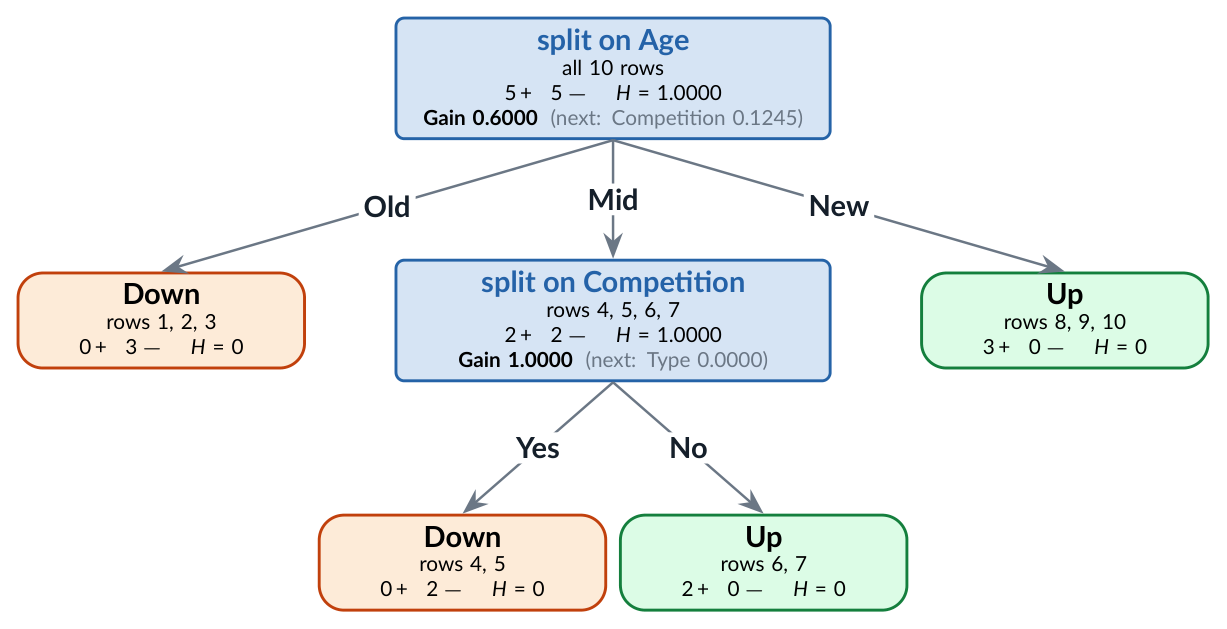
\includegraphics[width=412.0pt]{figs/c6_tree_profit.png}\end{center}
\par\Needspace{16\baselineskip}
% ch6fig:end

\hr

%=======================================================================
\T{6.N.6 Genetic algorithms: the method, then three runs}

\lead{The recipe every GA problem follows}
\begin{itemize}
  \item \textbf{1. Encode.} Say what one chromosome means, gene by gene. Almost every
        exam problem is a binary string with one bit per yes/no decision, or a string of
        digits.
  \item \textbf{2. Initialise.} Take the population the question gives you. If it gives
        none, write out four or five random strings and say they are random.
  \item \textbf{3. Evaluate.} Apply the fitness function to every chromosome, showing
        the substitution. \mk{An infeasible chromosome scores 0}, and
        saying \emph{why} it is infeasible earns the mark.
  \item \textbf{4. Select.} Rank them; keep the best, drop the worst.
  \item \textbf{5. Crossover.} State the point, draw the cut with a bar, write both
        offspring, and \textbf{evaluate them too}.
  \item \textbf{6. Mutate.} Flip one gene, say which, and evaluate.
  \item \textbf{7. Form the next generation} and compare its best and mean fitness
        against the previous one. \mk{That comparison is the answer};
        a GA solution without it is only half a solution.
\end{itemize}

%=======================================================================
\T{6.N.7 Problem 2.1 --- the knapsack, one full generation}

\begin{asked}[PROBLEM]{not a PYQ \textperiodcentered{} \emph{Insights} Example 6.1, the standard GA demonstration}
A thief has a knapsack of limited capacity that can hold almost 12 kg. Which items should
be kept in the knapsack so that its value is maximized? Solve using a genetic algorithm.
\par\penalty0\vspace{2pt}
\begin{tabularx}{0.44\linewidth}{@{}XXX@{}}
\hrow \thead{Item} & \thead{Weight} & \thead{Value} \\
A & 5 kg & \$12 \\
B & 3 kg & \$5 \\
C & 7 kg & \$10 \\
D & 2 kg & \$7 \\
\end{tabularx}
\end{asked}

\sbsr{0.50}{%
\lead{Step 1 \gap Chromosome encoding}
\begin{itemize}
  \item Four items, so a \textbf{4-bit chromosome} in the fixed order \code{A B C D}.
  \item Gene $=1$ means the item is in the knapsack, $0$ means it is not. The search
        space is $2^4 = 16$ chromosomes.
\end{itemize}
\lead{Step 2 \gap Initial population and fitness}
{\color{sub}\footnotesize Fitness $=$ total value if total weight $\leq 12$\,kg,
otherwise \textbf{0}.}
\begin{tabularx}{\linewidth}{@{}L{1.5cm}L{2.1cm}XXX@{}}
\hrow \thead{Chromo} & \thead{Items} & \thead{Weight} & \thead{Value} &
  \thead{Fitness} \\
$C_1$ 0010 & C       & 7 kg  & 10 & 10 \\
$C_2$ 0110 & B, C    & 10 kg & 15 & 15 \\
$C_3$ 1001 & A, D    & 7 kg  & 19 & \mk{19} \\
$C_4$ 1111 & A,B,C,D & \mk{17 kg} & 34 & \mk{0} \\
\end{tabularx}
\begin{itemize}
  \item $C_4$ is the heaviest \emph{and} the most valuable, and it scores \textbf{zero}:
        17 kg will not fit in a 12 kg sack, so it is not a solution at all.
  \item Generation 1: best $=19$, mean $=\frac{10+15+19+0}{4}=11.0$.
\end{itemize}}{%
\lead{Step 3 \gap Selection}
\begin{itemize}
  \item Rank: $C_3$ (19), $C_2$ (15), $C_1$ (10), $C_4$ (0).
  \item $C_4$ has zero fitness so a roulette wheel gives it \mk{no
        slice at all} and it never reproduces. Take $C_3$ and $C_2$ as parents.
\end{itemize}
\lead{Step 4 \gap Single-point crossover after gene 2}
\begin{tabularx}{\linewidth}{@{}L{2.4cm}L{2.2cm}XX@{}}
\hrow \thead{} & \thead{String} & \thead{Weight} & \thead{Fitness} \\
Parent $C_3$ & 1 0 $|$ 0 1 & 7 kg & 19 \\
Parent $C_2$ & 0 1 $|$ 1 0 & 10 kg & 15 \\
Offspring $O_1$ & 1 0 $|$ 1 0 & 12 kg & \mk{22} \\
Offspring $O_2$ & 0 1 $|$ 0 1 & 5 kg & 12 \\
\end{tabularx}
\begin{itemize}
  \item $O_1 = 1010$ is A and C: $5+7=12$ kg, exactly the capacity, value $12+10=22$.
        \mk{Better than either parent}, which is crossover doing its
        job.
\end{itemize}
\lead{Step 5 \gap Mutation}
\begin{itemize}
  \item Flip \textbf{gene 2} of $C_3=1001$: \code{1001 -> 1101}.
  \item $1101$ is A, B and D: $5+3+2=10$ kg, value $12+5+7=\mathbf{24}$.
\end{itemize}}

\sbs{%
\lead{Step 6 \gap Generation 2}
\begin{tabularx}{\linewidth}{@{}L{2.6cm}XXX@{}}
\hrow \thead{Chromosome} & \thead{Weight} & \thead{Value} & \thead{Fitness} \\
1101 (mutant) & 10 kg & 24 & \mk{24} \\
1010 ($O_1$)  & 12 kg & 22 & 22 \\
1001 ($C_3$)  & 7 kg  & 19 & 19 \\
0110 ($C_2$)  & 10 kg & 15 & 15 \\
\end{tabularx}
\begin{itemize}
  \item Best $19 \rightarrow \mathbf{24}$; mean $11.0 \rightarrow \mathbf{20.0}$. Both
        rose, which is what you must state.
  \item The two weakest of generation 1 ($C_1$ and the infeasible $C_4$) have been
        replaced by the offspring and the mutant.
\end{itemize}}{%
\par\penalty0\vspace{2pt}
\noindent\colorbox{gdL}{\parbox{\dimexpr\linewidth-2\fboxsep}{\textbf{Answer.} Take
\textbf{A, B and D}: 10 kg, value \textbf{\$24}. Chromosome \textbf{1101}.}}
\lead{Termination, and the point of the whole problem}
\begin{itemize}
  \item An exhaustive check of all 16 chromosomes confirms 24 is the
        \mk{global optimum}; the next best feasible sacks are 1010 and
        0111, both worth 22. So the run stops here, having converged.
  \item \mk{Notice which operator found it.} Crossover took 19 to 22.
        It could never have reached 24, because \emph{no chromosome in the population
        carried a 1 in gene B and gene D together} $-$ crossover can only shuffle genes
        that already exist. Mutation supplied the missing bit.
  \item That is the complete answer to \yr{\texttt{81 Ba}}'s \emph{``justify why mutation
        is important''}, and it is far stronger than quoting the definition.
\end{itemize}}

%=======================================================================
\T{6.N.8 Problem 2.2 --- fitness, ranking and crossover on eight-gene chromosomes}

\creamq{Rank the chromosomes by fitness, then perform the crossover operations}{\m{2+8}}
{\color{sub}\footnotesize \yr{\textbf{75 Bh}} \m{2+8} \gap$\cdot$\gap
\mk{the paper prints no chromosome list} $-$ the sentence ends and Q7
follows \gap$\cdot$\gap the four chromosomes below are the ones the standard version of
this question carries (\emph{Insights} Example 6.2) \gap$\cdot$\gap the swarm-intelligence
half of the question is answered in \S6.9 of the theory}

\begin{asked}{\textbf{75 Bh} \textperiodcentered{} Q6 \textperiodcentered{} \m{2+8}}
What do you understand by swarm intelligence? Suppose chromosomes are of the form
x $=$ a b c d e f g h with a fixed length of eight genes. Each gene can be any digit
between 0 and 9. Let the fitness of individual x be calculated as:
\par\penalty0\vspace{1pt}
\mbox{}\hfill $f(x) = (a+b) - (c+d) + (e+f) - (g+h)$ \hfill\mbox{}
\par\penalty0\vspace{1pt}
and let the initial population consist of four individuals with the following
chromosomes.
\par\penalty0\vspace{1pt}
{\color{sub}\footnotesize \mk{DEFECT IN THE PAPER}: the sentence ends
there and no chromosome list is printed. Confirmed against the scan. Worked below with
the standard four.}
\end{asked}

\begin{asked}[SUPPLIED]{the four chromosomes the textbook version of this question prints}
$x_1 = 65413532$ \gap $x_2 = 87126601$ \gap $x_3 = 23921285$ \gap $x_4 = 41852094$
\par\penalty0\vspace{1pt}
(a) Evaluate the fitness of each, and rank them fittest first.
\gap (b) Perform single-point crossover of the two fittest at the middle point, and a
two-point crossover of $x_1$ and $x_3$.
\end{asked}

\sbsr{0.53}{%
\lead{(a) Step 1 \gap Fitness of each chromosome}
{\color{sub}\footnotesize Read the eight digits as $a$ to $h$ in order, then substitute.}
\begin{tabularx}{\linewidth}{@{}L{0.9cm}L{2.1cm}XX@{}}
\hrow \thead{} & \thead{Chromosome} & \thead{Substitution} & \thead{$f(x)$} \\
$x_1$ & 6 5 4 1 3 5 3 2 & $(6{+}5)-(4{+}1)+(3{+}5)-(3{+}2)$ \newline
        $=11-5+8-5$ & 9 \\
$x_2$ & 8 7 1 2 6 6 0 1 & $(8{+}7)-(1{+}2)+(6{+}6)-(0{+}1)$ \newline
        $=15-3+12-1$ & \mk{23} \\
$x_3$ & 2 3 9 2 1 2 8 5 & $(2{+}3)-(9{+}2)+(1{+}2)-(8{+}5)$ \newline
        $=5-11+3-13$ & $-16$ \\
$x_4$ & 4 1 8 5 2 0 9 4 & $(4{+}1)-(8{+}5)+(2{+}0)-(9{+}4)$ \newline
        $=5-13+2-13$ & $-19$ \\
\end{tabularx}
\lead{Step 2 \gap Rank}
\par\penalty0\vspace{2pt}
\noindent\colorbox{gdL}{\parbox{\dimexpr\linewidth-2\fboxsep}{\textbf{Answer (a).}
Fittest first: $\mathbf{x_2\,(23)},\; x_1\,(9),\; x_3\,(-16),\; x_4\,(-19)$.
Mean fitness of generation 1 $= \frac{9+23-16-19}{4} = \mathbf{-0.75}$.}}
\begin{itemize}
  \item \mk{Read the fitness function before you compute}: genes
        $a,b,e,f$ are \emph{added} and $c,d,g,h$ are \emph{subtracted}, so a fit
        chromosome is large in positions 1, 2, 5, 6 and small in 3, 4, 7, 8. $x_2$ is
        exactly that shape; $x_4$ is its mirror image, and scores $-19$.
  \item The theoretical maximum is $f = 36$ at \code{99009900}, the minimum $-36$.
\end{itemize}}{%
\lead{(b) Step 3 \gap Single-point crossover of the two fittest, at the middle}
{\color{sub}\footnotesize Eight genes, so the middle point is after gene 4.}
\begin{tabularx}{\linewidth}{@{}L{1.9cm}L{2.5cm}XX@{}}
\hrow \thead{} & \thead{String} & \thead{Substitution} & \thead{$f$} \\
$x_2$ & 8712 $|$ 6601 & & 23 \\
$x_1$ & 6541 $|$ 3532 & & 9 \\
$O_1$ & 8712 $|$ 3532 & $15-3+8-5$ & 15 \\
$O_2$ & 6541 $|$ 6601 & $11-5+12-1$ & \mk{17} \\
\end{tabularx}
\begin{itemize}
  \item Both offspring beat $x_1$; neither beats $x_2$. \mk{Mean rises
        from $-0.75$ to $16$} if the two weakest are replaced by $O_1$ and $O_2$.
\end{itemize}
\lead{Step 4 \gap Two-point crossover of $x_1$ and $x_3$, cuts after genes 2 and 6}
\begin{tabularx}{\linewidth}{@{}L{1.9cm}L{2.9cm}XX@{}}
\hrow \thead{} & \thead{String} & \thead{Substitution} & \thead{$f$} \\
$x_1$ & 65 $|$ 4135 $|$ 32 & & 9 \\
$x_3$ & 23 $|$ 9212 $|$ 85 & & $-16$ \\
$O_1$ & 65 $|$ 9212 $|$ 32 & $11-11+3-5$ & $-2$ \\
$O_2$ & 23 $|$ 4135 $|$ 85 & $5-5+8-13$  & $-5$ \\
\end{tabularx}
\begin{itemize}
  \item In a two-point crossover the \textbf{middle segment} is exchanged and the two
        outer segments stay put.
  \item \mk{Both offspring are worse than $x_1$}, and that is worth
        stating: crossover does not guarantee improvement. It is \emph{selection},
        applied next generation, that throws these away and keeps the gains.
\end{itemize}}

%=======================================================================
\T{6.N.9 Problem 2.3 --- reaching a target fitness, and a textbook crossover that does nothing}

\begin{asked}[PROBLEM]{not a PYQ \textperiodcentered{} \emph{Insights} Example 6.3, reworked $-$ see the note}
You are given a coin. Find the generations using a genetic algorithm so that you can get
the number of heads above 30. Take 5 chromosomes made up of 10 genes to proceed with the
solution.
\end{asked}

\sbsr{0.50}{%
\lead{Steps 1 and 2 \gap Encoding and the initial population}
\begin{itemize}
  \item Ten tosses per chromosome: gene $1 =$ \textbf{head}, $0 =$ \textbf{tail}.
  \item Fitness of a chromosome $=$ its number of heads. The \emph{objective} is on the
        population: \mk{total heads $> 30$} across all five.
\end{itemize}
\begin{tabularx}{\linewidth}{@{}L{1.3cm}L{3.2cm}X@{}}
\hrow \thead{} & \thead{Chromosome} & \thead{$f =$ heads} \\
$C_1$ & 1 0 0 0 1 0 1 1 0 0 & 4 \\
$C_2$ & 1 1 1 0 0 1 0 1 1 0 & 6 \\
$C_3$ & 1 0 1 0 1 1 0 0 1 0 & 5 \\
$C_4$ & 0 1 1 1 1 0 1 0 1 1 & \mk{7} \\
$C_5$ & 0 1 1 1 0 0 1 1 1 1 & \mk{7} \\
\hrow \multicolumn{2}{@{}l}{\textbf{Total}} & \textbf{29} \gap
  {\color{sub}\footnotesize $< 30$, so continue} \\
\end{tabularx}
\lead{Step 3 \gap Selection}
\begin{itemize}
  \item The two fittest are $C_4$ and $C_5$, both 7. Take them as parents.
\end{itemize}
\lead{Step 4 \gap Choosing the crossover point matters here}
\begin{itemize}
  \item $C_4$ and $C_5$ \mk{share their first four genes}, \code{0111}.
        Cut anywhere in the first four positions and the ``offspring'' are just the two
        parents swapped $-$ no new chromosome exists and the population cannot improve.
  \item So cut \textbf{after gene 6}, where the parents actually differ.
\end{itemize}}{%
\begin{tabularx}{\linewidth}{@{}L{1.5cm}L{3.5cm}X@{}}
\hrow \thead{} & \thead{String} & \thead{$f$} \\
$C_4$ & 011110 $|$ 1011 & 7 \\
$C_5$ & 011100 $|$ 1111 & 7 \\
$O_1$ & 011110 $|$ 1111 & \mk{8} \\
$O_2$ & 011100 $|$ 1011 & 6 \\
\end{tabularx}
\lead{Step 5 \gap Generation 2: keep the best five of the seven}
\begin{tabularx}{\linewidth}{@{}L{3.4cm}XX@{}}
\hrow \thead{Chromosome} & \thead{$f$} & \thead{} \\
$O_1$ 0111101111 & \mk{8} & new best \\
$C_4$ 0111101011 & 7 & \\
$C_5$ 0111001111 & 7 & \\
$C_2$ 1110010110 & 6 & \\
$O_2$ 0111001011 & 6 & \\
\hrow \textbf{Total} & \textbf{34} & \\
\end{tabularx}
\par\penalty0\vspace{2pt}
\noindent\colorbox{gdL}{\parbox{\dimexpr\linewidth-2\fboxsep}{\textbf{Answer.} Total
heads $29 \rightarrow \mathbf{34}$, and the best individual $7 \rightarrow \mathbf{8}$.
The objective is reached in the \textbf{second generation}.}}
\lead{\mk{Where the textbook goes wrong, and why it matters}}
\begin{itemize}
  \item \emph{Insights} crosses the same two parents \emph{inside} the four genes they
        share, so its $O_1$ and $O_2$ come out equal to $C_5$ and $C_4$. Its total still
        reaches 34, but only because the best chromosome has been \textbf{counted
        twice}; the best individual never improves past 7.
  \item Cutting where the parents differ produces a genuinely new chromosome with 8
        heads. \mk{An examiner reading the two solutions can see which
        one understood crossover.}
\end{itemize}}

\hr

%=======================================================================
\T{6.N.10 Problem 3.1 --- fuzzy set operations}

\begin{asked}[PROBLEM]{not a PYQ directly, but the arithmetic behind every ``explain fuzzy operations'' answer}
For the fuzzy sets
$A = \{(10,\,0.2),\,(20,\,0.3),\,(30,\,0.4),\,(40,\,0.5)\}$ and
$B = \{(10,\,0.3),\,(20,\,0.4),\,(30,\,0.1),\,(40,\,0.2)\}$
over the universe $U = \{10, 20, 30, 40\}$, find
$A \cup B$, $A \cap B$, $A'$, the bold union $A \oplus B$ and the bold intersection
$A \odot B$.
\end{asked}

\sbsr{0.62}{%
\lead{Work element by element}
{\color{sub}\footnotesize Every fuzzy operation is defined \emph{pointwise}: apply it to
the membership values at each $x$ independently. There is nothing else to it.}
\begin{tabularx}{\linewidth}{@{}L{3.6cm}XXXX@{}}
\hrow \thead{$x$} & \thead{10} & \thead{20} & \thead{30} & \thead{40} \\
$\mu_A(x)$ & 0.2 & 0.3 & 0.4 & 0.5 \\
$\mu_B(x)$ & 0.3 & 0.4 & 0.1 & 0.2 \\
\hrow $A \cup B = \max$ & 0.3 & 0.4 & 0.4 & 0.5 \\
$A \cap B = \min$ & 0.2 & 0.3 & 0.1 & 0.2 \\
$A' = 1-\mu_A$ & 0.8 & 0.7 & \mk{0.6} & 0.5 \\
$A \oplus B = \min(1, \mu_A{+}\mu_B)$ & 0.5 & 0.7 & 0.5 & 0.7 \\
$A \odot B = \max(0, \mu_A{+}\mu_B{-}1)$ & 0 & 0 & 0 & 0 \\
\end{tabularx}
\begin{itemize}
  \item \textbf{Bold intersection is empty} because no pair of memberships sums past 1.
        Say that; it is the check that you applied the formula rather than guessing.
  \item \mk{Note $A \cap A' \neq \emptyset$}: at $x=40$ both are 0.5,
        so their intersection is 0.5. In crisp set theory that is impossible. This one
        line is the sharpest possible answer to \emph{``how does fuzzy logic differ from
        classical logic''}, and the same goes for $A \cup A' \neq U$.
\end{itemize}}{%
\par\penalty0\vspace{2pt}
\noindent\colorbox{gdL}{\parbox{\dimexpr\linewidth-2\fboxsep}{\textbf{Answers.}\\
$A \cup B = \{(10,0.3),(20,0.4),(30,0.4),(40,0.5)\}$\\
$A \cap B = \{(10,0.2),(20,0.3),(30,0.1),(40,0.2)\}$\\
$A' = \{(10,0.8),(20,0.7),(30,0.6),(40,0.5)\}$\\
$A \oplus B = \{(10,0.5),(20,0.7),(30,0.5),(40,0.7)\}$\\
$A \odot B = \{(10,0),(20,0),(30,0),(40,0)\}$}}
\lead{\mk{One correction to the textbook}}
\begin{itemize}
  \item \emph{Insights} p167 prints the complement as
        $A' = \{(10,0.8),(20,0.7),(30,\mathbf{0.5}),(40,0.5)\}$.
  \item $\mu_A(30) = 0.4$, so $1 - 0.4 = \mathbf{0.6}$, not 0.5. Every other value in
        that box is right; only this one is a slip.
  \item The check that catches it in one second: \mk{$\mu_A(x) +
        \mu_{A'}(x)$ must equal exactly 1 at every element}. Run it down the
        column before you hand the paper in.
\end{itemize}}

%=======================================================================
\T{6.N.11 Problem 3.2 --- fuzzification: turning a crisp reading into a membership}

\begin{asked}[PROBLEM]{not a PYQ \textperiodcentered{} \emph{Insights} p166, the step every fuzzy question needs}
The linguistic term \emph{medium speed} has a membership function that rises linearly
from 0 at 7.5 km/h to 1 at 12.5 km/h. Fuzzify the readings 10 km/h and 9 km/h.
\end{asked}

\sbs{%
\lead{The one formula}
{\color{sub}\footnotesize On a rising limb from $a$ to $b$:}
\[ \mu(x) = \frac{x-a}{b-a} \qquad a \leq x \leq b \]
\begin{itemize}
  \item \textbf{At 10 km/h}:
        $\mu = \dfrac{10-7.5}{12.5-7.5} = \dfrac{2.5}{5} = \mathbf{0.5}$, so the fuzzy
        pair is $(10,\ 0.5)$.
  \item \textbf{At 9 km/h}:
        $\mu = \dfrac{9-7.5}{5} = \dfrac{1.5}{5} = \mathbf{0.3}$, so the pair is
        $(9,\ 0.3)$.
  \item On a \emph{falling} limb from $b$ to $c$ the formula is
        $\mu(x) = \frac{c-x}{c-b}$, and a triangle is one of each.
\end{itemize}}{%
\lead{Two things this small problem teaches}
\begin{itemize}
  \item \mk{The first number in the pair is the element, not the
        peak.} \emph{Insights} writes the second answer as $(10,\,0.3)$, but the
        reading was 9 km/h, so the pair is $(9,\,0.3)$. The membership value is right;
        the label is not.
  \item A crisp reading normally fuzzifies to \mk{more than one
        term at once}, because the membership functions overlap: 10 km/h might be
        \emph{slow} to degree 0.5 and \emph{medium} to degree 0.5 at the same time. That
        overlap is the whole reason fuzzy control is smooth, so never report only one
        term unless the reading really is outside every other set.
\end{itemize}}

%=======================================================================
\T{6.N.12 Problem 3.3 --- a complete Mamdani fuzzy inference}

{\color{sub}\footnotesize \mk{Which fuzzy answer does this paper want?} Sixteen papers ask
something about fuzzy logic and they do not want the same answer. Decide from
\emph{what is asked for}, not from the word \emph{fuzzy}.
\textbf{``explain fuzzy inference / the Mamdani method / the steps, with an example''},
5 marks or more $\rightarrow$ \S6.N.12, the worked run below.
\textbf{``the architecture''}, or \textbf{``the major steps for developing a system based
on fuzzy logic''} $\rightarrow$ \S6.N.13: those ask you to \emph{build} the variables,
membership functions and rule base that \S6.N.12 is handed for free.
\textbf{A 4-mark short note, or a 2-mark ``what is fuzzy logic''} $\rightarrow$ neither of
them. That is \textbf{Ch 6 \S6.7}, and running a defuzzification for it spends twenty
minutes earning four marks.}

\creamq{Explain fuzzy inference / the Mamdani method / the steps of a fuzzy inference system, with an example}{\m{1+2+5}\m{2+6}\m{3+7}\m{8}}
{\color{sub}\footnotesize \tF{6} \yr{73 Ma \m{3+7}, \textbf{\texttt{80 Bh}} \m{8},
\textbf{\texttt{79 Bh}} \m{2+6}, 70 Ma \m{2+6}, 80 Ash \m{1+2+5}, 79 Ash \m{1+2+5}}
\gap$\cdot$\gap the papers never supply numbers, so \mk{you have to
invent the example} $-$ this one is small enough to write out in full in about
ten minutes \gap$\cdot$\gap \yr{73 Ma} is the only paper in the 41 that names
\textbf{Mamdani}; the other five say only \emph{fuzzy inference} or \emph{the steps},
and this one run answers all six}

\begin{asked}{73 Ma \textperiodcentered{} Q7 \textperiodcentered{} \m{3+7}}
What is Fuzzy Logic and why is it important? Explain the Mamdani Fuzzy Inference Method
with example.
\end{asked}

\begin{asked}[PROBLEM]{the worked example, chosen so every number is checkable}
A fan-speed controller has two inputs, temperature $T$ (0--40 $^\circ$C) and humidity
$H$ (0--100 \%), and one output, fan speed $S$ (0--100 \%).
\par\penalty0\vspace{1pt}
\textbf{Membership functions.} \emph{Cold}: 1 up to 10, falling to 0 at 20.
\emph{Warm}: triangle 10--20--30. \emph{Hot}: 0 at 20, rising to 1 at 30 and staying
there. \emph{Low humidity}: 1 up to 30, falling to 0 at 60. \emph{High humidity}: 0 at
30, rising to 1 at 60. Output sets \emph{Slow}, \emph{Medium}, \emph{Fast} are triangles
peaking at 0, 50 and 100.
\par\penalty0\vspace{1pt}
\textbf{Rules.} R1: IF $T$ is Cold AND $H$ is Low THEN $S$ is Slow.
R2: IF $T$ is Warm THEN $S$ is Medium.
R3: IF $T$ is Hot OR $H$ is High THEN $S$ is Fast.
\par\penalty0\vspace{1pt}
Find the fan speed for $T = 26\,^\circ$C and $H = 45\,\%$.
\end{asked}

\sbsr{0.50}{%
\lead{Step 1 \gap Fuzzify both inputs}
{\color{sub}\footnotesize Read each crisp value off every membership curve it touches.}
\begin{tabularx}{\linewidth}{@{}L{2.0cm}XX@{}}
\hrow \thead{Term} & \thead{Working at $T=26$, $H=45$} & \thead{$\mu$} \\
Cold  & $26 > 20$, outside the set & 0 \\
Warm  & falling limb: $\frac{30-26}{30-20}$ & \mk{0.4} \\
Hot   & rising limb: $\frac{26-20}{30-20}$ & \mk{0.6} \\
Low   & falling limb: $\frac{60-45}{60-30}$ & 0.5 \\
High  & rising limb: $\frac{45-30}{60-30}$ & 0.5 \\
\end{tabularx}
\begin{itemize}
  \item 26\,$^\circ$C is \mk{both warm and hot}, and 45\,\% is equally
        low and high. That is the point of fuzzy logic: no reading has to pick a side.
  \item Check: $\mu_{Warm} + \mu_{Hot} = 1$ and $\mu_{Low} + \mu_{High} = 1$, as they
        must be where exactly two curves overlap linearly.
\end{itemize}
\lead{Step 2 \gap Fire the rules \gap{\color{sub}\footnotesize(AND $=$ min, OR $=$ max)}}
\begin{tabularx}{\linewidth}{@{}L{0.9cm}XX@{}}
\hrow \thead{Rule} & \thead{Strength} & \thead{$w$} \\
R1 & $\min(\mu_{Cold},\ \mu_{Low}) = \min(0,\ 0.5)$ & \mk{0} \\
R2 & $\mu_{Warm}$ & 0.4 \\
R3 & $\max(\mu_{Hot},\ \mu_{High}) = \max(0.6,\ 0.5)$ & 0.6 \\
\end{tabularx}
\begin{itemize}
  \item \textbf{R1 does not fire at all} ($w=0$), so \emph{Slow} contributes nothing.
        Saying so explicitly is worth a mark.
\end{itemize}}{%
\lead{Step 3 \gap Implication: clip each output set at its rule strength}
\begin{itemize}
  \item \emph{Medium} is clipped at \textbf{0.4}, \emph{Fast} at \textbf{0.6}. Mamdani
        implication is the \textbf{min} operator, so the top of each triangle is simply
        cut flat.
\end{itemize}
\lead{Step 4 \gap Aggregation: take the max of the clipped sets}
{\color{sub}\footnotesize Sample the aggregated set every 10 units of $S$.}
\begin{tabularx}{\linewidth}{@{}L{2.3cm}XXXXXX@{}}
\hrow \thead{$S$} & 0 & 10 & 20 & 30 & 40 & 50 \\
clipped Medium & 0 & 0.2 & 0.4 & 0.4 & 0.4 & 0.4 \\
clipped Fast & 0 & 0 & 0 & 0 & 0 & 0 \\
\hrow \thead{aggregate} & 0 & 0.2 & 0.4 & 0.4 & 0.4 & 0.4 \\
\hrow \thead{$S$} & 60 & 70 & 80 & 90 & 100 & \\
clipped Medium & 0.4 & 0.4 & 0.4 & 0.2 & 0 & \\
clipped Fast & 0.2 & 0.4 & 0.6 & 0.6 & 0.6 & \\
\hrow \thead{aggregate} & 0.4 & 0.4 & \mk{0.6} & \mk{0.6} &
  \mk{0.6} & \\
\end{tabularx}
\lead{Step 5 \gap Defuzzify by the centre of gravity}
\[ S^{*} = \frac{\sum S_i\, \mu(S_i)}{\sum \mu(S_i)}
        = \frac{272}{4.4} = \mathbf{61.8\,\%} \]
{\color{sub}\footnotesize $\sum \mu = 0+0.2+0.4+0.4+0.4+0.4+0.4+0.4+0.6+0.6+0.6 = 4.4$;
$\sum S\mu = 2+8+12+16+20+24+28+48+54+60 = 272$. Integrating the true area instead of
sampling gives 58.8 \%, so the ten-point sum is accurate to about 3 \%, which is well
inside what any examiner expects.}}

\sbs{%
\par\penalty0\vspace{2pt}
\noindent\colorbox{gdL}{\parbox{\dimexpr\linewidth-2\fboxsep}{\textbf{Answer.} Run the
fan at \textbf{about 62 \%}. Rules R2 and R3 fired at 0.4 and 0.6; R1 did not fire.}}
\lead{The six Mamdani operations, named against the steps above}
\begin{itemize}
  \item \textbf{1. Determine the rules} $-$ R1, R2, R3, given.
  \item \textbf{2. Fuzzify the inputs} $-$ Step 1.
  \item \textbf{3. Combine to get rule strength} $-$ Step 2, fuzzy AND $=$ min,
        OR $=$ max.
  \item \textbf{4. Implication} $-$ Step 3, clip each consequent set at its strength.
  \item \textbf{5. Aggregation} $-$ Step 4, union the clipped sets with max.
  \item \textbf{6. Defuzzification} $-$ Step 5, centre of gravity.
\end{itemize}}{%
\lead{The shortcut, and when it is safe}
\begin{itemize}
  \item If you are short of time, the \textbf{weighted average of the consequent peaks}
        is one line:
  \[ S^{*} = \frac{0.4(50) + 0.6(100)}{0.4+0.6} = \frac{80}{1.0} = 80\,\% \]
  \item \mk{It is not the same answer}, because it ignores the shape
        and the overlap of the two output sets. Use it only when the question says
        \emph{weighted average} or \emph{centre of sums}; if it says
        \textbf{centroid} or \textbf{centre of gravity}, do the sampled sum above.
  \item \mk{Two checks before you write the final number}: the answer
        must lie \emph{inside} the output range (0--100 here), and it must sit between
        the peaks of the sets that fired (50 and 100). Both 61.8 and 80 pass; a number
        outside that band means an arithmetic slip.
\end{itemize}}

%=======================================================================
\T{6.N.13 Problem 3.4 --- designing the fuzzy system that Problem 3.3 runs}

\creamq{What are the major steps for developing a system based on fuzzy logic? Explain the architecture and working mechanism of a fuzzy inference system}{\m{2+5}\m{2+6}}
{\color{sub}\footnotesize \tP{2} \yr{\textbf{80 Ch} \m{2+5}, \texttt{82 Ba} \m{2+6}}
\gap$\cdot$\gap \mk{these two do not want a defuzzification}: \S6.N.12
is handed its membership functions and its three rules, and these papers ask
\emph{where those came from} \gap$\cdot$\gap the 2-mark opener,
\emph{when do we use fuzzy logic}, is the list in \textbf{Ch 6 \S6.7}}

\begin{asked}{\textbf{80 Ch} \textperiodcentered{} Q7 \textperiodcentered{} \m{2+5}}
When shall we use Fuzzy Logic? Explain with an appropriate example. What are the major
steps for developing a system based on Fuzzy logic?
\end{asked}

\begin{asked}{\texttt{82 Ba} \textperiodcentered{} Q7 \textperiodcentered{} \m{2+6}}
When do we use fuzzy logic? Explain the architecture and working mechanism of a fuzzy
inference system.
\end{asked}

\sbsr{0.47}{%
\lead{The seven design steps, in the order you do them}
\begin{enumerate}
  \item \textbf{Confirm fuzzy logic fits.} Expert rules exist, no exact plant model does,
        and the boundaries are linguistic. If a threshold already works, do not fuzzify it.
  \item \textbf{Name the variables and their universes of discourse.} One per sensor and
        one per actuator, each with the range it physically spans.
  \item \textbf{Choose the linguistic terms} for each variable. Three to five per
        variable; \mk{the rule count is the product}, so five terms on
        three inputs is 125 rules and unmaintainable.
  \item \textbf{Draw one membership function per term.} Triangles and trapezoids, and
        \mk{they must overlap}: every point of the universe belongs to
        at least one set, and neighbours cross at about 0.5.
  \item \textbf{Build the rule base} as a matrix of every input-term combination against
        the action to take. The domain expert fills the cells, not the engineer.
  \item \textbf{Fix the operators}: AND $=$ min, OR $=$ max, implication $=$ min
        (Mamdani), aggregation $=$ max, and pick the defuzzifier (centroid unless the
        question says otherwise).
  \item \textbf{Simulate, tune, iterate.} Run known cases, move the membership breakpoints
        until the outputs match the expert's judgement, then deploy.
\end{enumerate}
{\color{sub}\footnotesize Steps 1--5 are design and happen once. Steps 4 and 6 are what the
running system executes on every reading $-$ that is the \emph{working mechanism} half of
\yr{\texttt{82 Ba}}, and its block diagram is the architecture figure in
\textbf{\S6.7}.}}{%
\lead{Worked \gap step 2--4 for the fan controller of \S6.N.12}
\begin{tabularx}{\linewidth}{@{}L{1.5cm}L{2.1cm}X@{}}
\hrow \thead{Variable} & \thead{Universe} & \thead{Terms, and where they cross} \\
$T$ in & 0--40 $^\circ$C & Cold, Warm, Hot. Cold/Warm cross at \mk{15},
  Warm/Hot at \mk{25}, both at $\mu = 0.5$ \\
$H$ in & 0--100 \% & Low, High, crossing at \mk{45} \\
$S$ out & 0--100 \% & Slow, Medium, Fast, peaking at 0, 50, 100 \\
\end{tabularx}
\begin{itemize}
  \item \mk{This is why \S6.N.12 read $\mu_{Low} = \mu_{High} = 0.5$}:
        its 45 \% is exactly the crossover you placed here. A reading that lands on a
        crossover is the best sanity check a design gets.
\end{itemize}
\lead{Step 5 \gap The rule matrix, all six cells}
\begin{tabularx}{\linewidth}{@{}L{1.4cm}XX@{}}
\hrow \thead{} & \thead{$H$ Low} & \thead{$H$ High} \\
$T$ Cold & Slow & Fast \\
$T$ Warm & Medium & Medium \emph{and} Fast \\
$T$ Hot & Fast & Fast \\
\end{tabularx}
\begin{itemize}
  \item \mk{The Warm/High cell naming two actions is not a bug.} Both
        fire, at their own strengths, and aggregation settles it. A crisp rule base would
        have to pick one and would jerk at the boundary.
\end{itemize}}

\sbsr{0.47}{%
\lead{\mk{The compression \S6.N.12 uses is not a relabelling}}
\begin{itemize}
  \item Whole rows and columns of that matrix agree, so it is tempting to write
        \emph{Hot \textbf{OR} High $\rightarrow$ Fast} as one rule and be done. That is
        what \S6.N.12's R3 does.
  \item \textbf{It changes the numbers.} A matrix cell fires at
        $\min(\mu_T, \mu_H)$, so a fully high humidity is dragged down by a
        half-cold temperature. An OR rule takes $\max$, and lets either antecedent
        carry the rule on its own.
\end{itemize}
\begin{tabularx}{\linewidth}{@{}L{3.5cm}XX@{}}
\hrow \thead{At $T=26$, $H=45$} & \thead{3 OR rules} & \thead{6 cells} \\
Slow & 0 & 0 \\
Medium & 0.4 & 0.4 \\
Fast & \mk{0.6} & \mk{0.5} \\
\hrow \thead{centroid} & \mk{61.8 \%} & \mk{59.8 \%} \\
\end{tabularx}}{%
\begin{itemize}
  \item Over the whole input grid the two rule bases give different firing strengths at
        \textbf{1386 of the 4141} integer $(T, H)$ points, and they are furthest apart at
        \mk{$T=15$, $H=60$}: the OR rule fires Fast at \textbf{1.0}
        because the air is fully humid, the matrix at \textbf{0.5} because
        $\min$ sees a temperature that is only half cold.
  \item \mk{Which one to write}: either, but \textbf{say which}. The
        marks are for naming the operators and using them consistently, not for the
        crisp number $-$ no paper in the 41 supplies data, so no paper has a right
        answer to compare against.
  \item \textbf{Do not print the matrix and then solve with the OR rules without a word},
        which is the one version that is simply inconsistent.
\end{itemize}}

\sbs{%
\par\penalty0\vspace{2pt}
\noindent\colorbox{gdL}{\parbox{\dimexpr\linewidth-2\fboxsep}{\textbf{Answer.} Seven
steps: confirm the fit, name the variables and their ranges, choose linguistic terms,
draw overlapping membership functions, fill the rule matrix, fix the operators and the
defuzzifier, then simulate and tune. \textbf{Design ends where \S6.N.12 begins.}}}}{%
\lead{\mk{What loses marks here}}
\begin{itemize}
  \item \textbf{Answering with a defuzzification.} Neither paper gives numbers, and
        neither asks for a crisp output. Five or six marks are for the \emph{procedure}.
  \item \textbf{Membership functions that do not overlap.} Then the system is a lookup
        table with fuzzy notation, and it jerks at every boundary. Say the overlap is
        deliberate.
  \item \textbf{Forgetting the 2-mark opener.} Both papers open with \emph{when do we use
        fuzzy logic}, and it is a separate list: vague boundaries, expert rules available,
        no mathematical model, tolerance for imprecision. \textbf{\S6.7}.
\end{itemize}}

\hr

\lead{Sources and verification}
\begin{itemize}
  \item All three PYQ data tables are transcribed from
        \code{AI/ocr/CT-653\_CT-710\_CT-78506\_NewScan\_OCR.md}, cell by cell.
  \item Method throughout follows \emph{Insights on Artificial Intelligence} ch\,6,
        checked independently. \mk{Two of its numbers are wrong and are
        corrected here}: the complement in Problem 3.1 and the element label in
        Problem 3.2. \mk{One of its methods is wrong}: the crossover in
        Problem 2.3.
  \item Every entropy, gain, fitness, membership and defuzzified value on these pages is
        recomputed from the problem statement by \code{verify.py}, which also proves the
        knapsack optimum by exhaustive search over all 16 chromosomes and confirms that
        \emph{Insights}' crossover point produces offspring identical to its parents.
\end{itemize}
